\documentclass[12pt]{article}
\usepackage{xcolor}
\usepackage{listings}
\usepackage{apacite}
\usepackage{url}
\usepackage{amsmath}
\usepackage{amssymb}
\usepackage{tcolorbox}
\usepackage{tabularx}
\usepackage{tikz}
\usepackage{algorithm}
\usepackage{algorithmicx}
\usepackage{algpseudocodex}
\usepackage{longtable}
\tcbuselibrary{breakable}

% Recipe: pdflatex -> bibtex -> pdflatex*2

% Code listings
% Basic color definitions
\definecolor{codebg}{RGB}{245,245,245}
\definecolor{keyword}{RGB}{0,0,255}
\definecolor{comment}{RGB}{34,139,34}
\definecolor{string}{RGB}{170,55,241}

\lstset{
    basicstyle=\ttfamily\scriptsize,
    columns = fullflexible,
    backgroundcolor=\color{codebg},         
    commentstyle=\color{comment},
    keywordstyle=\color{keyword},
    stringstyle=\color{string},
    numbers=left,
    numberstyle=\tiny\color{gray},
    stepnumber=1,
    numbersep=8pt,
    showstringspaces=false,
    breaklines=true,
    frame=single,
    rulecolor=\color{gray!50},
    framesep=5pt,
    xleftmargin=15pt,
    tabsize=4,
    language=C++ % Default language
}

\title{\textbf{Exploring and comparing different merging algorithms for balanced binary search trees}}
\author{Changhui (Eric) Zhou}
\date{\today}

\begin{document}

\begin{titlepage}
    \maketitle
    \centering 

    IB Computer Science Extended Essay

    Word Count: 3150 (Oct 8 version)
\end{titlepage}

\tableofcontents
\clearpage

\section{Introduction}

A \textit{data structure} is a way to store and organize data in order to facilitate access and modifications \cite{CLRS}. Designing and choosing more efficient data structures has always been a great persuit for computer scientists, for optimal data structures can save huge amount of computing resources, especially in face of large amount of data. Basic data structures include ordered data structures like arrays, linked lists and binary search trees and unordered data structures like hashtables or disjoint set unions (DSU). 

For ordered data structures, merging two or more instances of them while maintaining its ordered property may be frequently used in practice. For example, to investigate the factors affacting the school grade, data from different schools may be grouped and merged according to various factors. The efficiency of combination varies significantly based on the data structure itself and the algorithm used in the process.  The merging of some data structures like linked lists, DSUs or heaps (especially leftist heaps) is simple and straightforward. However, these easy-to-merge data structures can lack of properties like random accessing (for linked lists or heaps) or ordered property (for DSUs). Balanced BSTs, however, supports a wide range of oprations in just $O(\log n)$ time, and is widely used in theoretical researches, competitions and real life applications.

This essay will focus on invesitgating the theoretical time complexity (usually described using big-O notation, showing the asymptotic upper bound \cite{CLRS}) and actual performance of merging algorithms of balanced BSTs, which are one of the most common and powerful data structure in real life. 

\textbf{Research question: How does different algorithm affect the efficiency of merging two instances of balanced search trees?}

\section{Theory}

\subsection{Data structure terminology}

When a homogeneous relation (a binary relation between two elements) $\le$ on a set of elements $X$ satisfies:

\begin{align*}
&\text{1. Antisymmetry:} && \forall u, v \in X, (u \le v \land v \le u) \Leftrightarrow u = v. \\
&\text{2. Totality:} && \forall u, v \in X, u \le v \lor v \le u. \\
&\text{3. Transitivity:} && \forall u, v, w \in X, (u \le v \land v \le w) \Rightarrow u \le w.\\
\end{align*}

We say $P = (X, \le)$ is a total order. For example $P = (\mathbb{R}, \le)$, where $\le$ is numerical comparison, is a total order. The set of finite strings and lexographical order comparison is also a total order. But $P = (\{S: S\subset \mathbb{R}\}, \subset)$ (i.e. all the real number sets and the subset relation) is not a total order.

Ordered data structures can store elements that satisfies a total order while maintaining their order. In C++, arrays, vectors, linked lists and sets can be ordered data structures, but unordered sets (hashtables) are not ordered data structures.

\begin{tcolorbox}[title=Definition]
    Ordered data structures are data structures that can store elements that satisfies a total order while maintaining their order.
\end{tcolorbox}

\subsection{Balanced binary search trees}

\begin{itemize} %might need to define edge, path, cycle, root, children, parent, subtree(?)
    \item A \textit{graph} $G = (V, E)$ is the combination of the vertex set $V$ and the edge set $E$.
    \item A \textit{tree} $T = (V, E)$ is a connected acylic graph.
            \begin{itemize}
                \item The \textit{root} of a tree is a designated vertex that has no parent. For every other vertex, exactly one of its neighbors is its parent. It can be easily proven that once the root is chosen, the tree is determined.
                \item The \textit{children} of a vertex are all its neighbors except for its parent. It can be easily proven that the parent of all the children of a vertex is the vertex itself.
                \item The \textit{leaf} of a tree is a vertex that has no children.
                \item The \textit{subtree} of a vertex $v$ is the union of $v$ and the subtree of all its children, or only the vertex itself in the case that $v$ is a leaf.
                \item The \textit{depth} of a tree or a subtree is the maximum number of edges on the simple path from the root to one of the leaves.
            \end{itemize}
    \item A \textit{binary tree} is a tree that has no more than two children for each node.
    \item A \textit{binary search tree (BST)} is a binary tree, whose nodes contain values under a total order, that has the following property: For any node $v$, all nodes in its left subtree are less than $v$, and all nodes in its right subtree are greater than $v$ \cite{CLRS}.
\end{itemize}

Generally speaking, a balanced BST is a BST whose depth or the cost of iterating from the root to one specific leaf is strictly, expectedly or amortized $O(\log n)$. There are different kinds of balanced BSTs, like splay tree, treap, AVL trees, scapegoat trees and red-black trees.

In this essay, we will focus on AVL trees (named after Adelson-Velsky and Landis). AVL trees are a type of self-balancing binary search trees, which adjusts its shape through rotations and maintain the difference of the depths of two subtrees at most one \cite{avl}\footnote{We assume the maximum depth difference is $1$ in this essay, which might not be the case in early studies.}.  AVL trees are chosen because their properties make it easy to implement and analyze. AVL trees are known to have simple, straightforward balancing condition. Unlike splay or treap, each opration on an AVL tree have a predictable time complexity for every operation, as the shape of the tree is relatively static. All the rebalance operations happen locally, and no case-heavy analysis (like in red-black tree) or amortized oprations (like in splay tree) are needed.



In this essay, we will assume that there are two instances of AVL trees $T_1$ and $T_2$ to be merged. Without losing generality, we will assume $T_1$ has $n$ elements and $T_2$ has $m$ elements and $n \ge m$.

% Perhaps more on data structures here. 

% Perhaps give what is already supported by avl trees. 

\subsection{Insertion-based merge}

One of the basic operations supported by a balanced BST is insertion, where one element is added to the tree and the order of the tree is automatically maintained. In fact, merging two instances of BSTs can be reduced to a sequence of insertions to a balanced BST. To be more specific, we iterate through all the elements in $T_2$, insert them one by one into $T_1$, that would be $m$ operations with each having time complexity of $O(\log n)$, resulting in a overall complexity of $O(m\log n)$. 

\begin{tcolorbox}[colback=orange!5!white, colframe=orange!75!black, title=Algorithm: Insertion-Based Merge]
\begin{algorithmic}[1]
\Require Two balanced binary search trees $T_1$ and $T_2$
\Ensure A single balanced binary search tree containing all elements from $T_1$ and $T_2$
\Procedure{InsertionBasedMerge}{$T_1, T_2$}
    \ForAll{elements $x$ in $T_2$ (in-order traversal)}
        \State \Call{$T_1.$ Insert}{$x$}
    \EndFor
    \State \Return $T_1$
\EndProcedure
\end{algorithmic}
\end{tcolorbox}

This algorithm performs well when $m/n$ is small, as the overall time complexity will be mainly $O(\log n)$. However, when $m$ and $n$ are relatively at the same scale, the overall time complexity will be close to $O(n\log n)$.

\subsection{In-order traversal merge}

Another way to merge two instances of BSTs is to utilize the property that each instance is already in-order. To combine them, we can view this process as merging two sorted subarrays into a new array, just like a merge sort. The iteration and new array construction process take $O(n+m)$ time. With proper construction function, we can create a balanced BST in linear time out of a sorted array. Therefore, the overall time complexity is $O(n+m)$.

\begin{tcolorbox}[colback=orange!5!white, colframe=orange!75!black, title=Algorithm: In-order traversal merge]
\begin{algorithmic}[1]
\Require Two balanced binary search trees $T_1$ and $T_2$
\Ensure A single balanced binary search tree containing all elements from $T_1$ and $T_2$
\Procedure{MergeSortBasedMerge}{$T_1, T_2$}
    \State $A_1 \gets$ \Call{InOrderTraversal}{$T_1$}
    \State $A_2 \gets$ \Call{InOrderTraversal}{$T_2$}
    \State $A \gets$ \Call{MergeSortedArrays}{$A_1, A_2$}
    \State $T \gets$ \Call{BuildBalancedBST}{$A$}
    \State \Return $T$
\EndProcedure
\end{algorithmic}
\end{tcolorbox}

This algorithm performs well when $m/n$ is large, as the overall time complexity will be approximately $O(n)$. However, when $m$ is pretty negeligible compared to $n$, a full iteration over $T_1$ will be still needed and the overall time complexity will still be $O(n)$, which wastes a lot of time.

In fact, it Stockmayer and Yao has proven that in term of number of comparisions, this algorithm is optimal when $m\le n\le \lfloor 3m/2 \rfloor +1$ \cite{stockmeyer1980optimality}. This algorithm, however, does not perform well outside this range. 

\subsection{Brown and Tarjan's merging algorithm (1979)}

In 1979, Brown and Tarjan proposed another algorithm based on the two merging algorithm mentioned above. It utilized both the tree structure for fast insertion-place location and the ordered property to reduce redundent operations. The algorithm again chooses the $T_1$ as the base tree and view the merging process as $m$ insertions to a balanced BST of size $n$. However, the property that the inserted objects themselves are sorted helped to make the algorithm more efficient. Instead of iterating from the root, each insertion starts with the ending position of the last insertion, as it can be already told that the next insertion will happen to the right of the last insertion. 

To be more specific, the algorithm keeps a stack called \textit{path} and a stack called \textit{successor}. The former is used to record the path from the root to the current node, while the latter records all the nodes on the \textit{path} that is larger than the current node (that means they are on the right side of the current node their left children is visited on the \textit{path}). Each insertion, instead of starting from the root, starts from the last node on the \textit{successor} that is smaller than the node to be inserted. Keep extending the \textit{path} and \textit{successor} during insertion. And the path shrinks back after the insertion, until a rebalance operation is triggered or we know that there need no rebalancing at all.

It is worth noticing that the rebalance operation may make the initial path unusable. In this case, we can simply dispose of the path under the rotated node start next insertion there \cite{brown1979fast}. 

\begin{tcolorbox}[breakable, colback=orange!5!white, colframe=orange!75!black, title=Algorithm: Brown and Tarjan's Merging Algorithm]
\begin{algorithmic}[1]
\Require Two balanced binary search trees $T_1$ (size $n$) and $T_2$ (size $m$), where $n \ge m$
\Ensure A single balanced BST containing all elements from $T_1$ and $T_2$
\Procedure{FastMerge}{$T_1, T_2$}
    \State Initialize stack \textit{path} $\gets$ \{root($T_1$)\}
    \State Initialize empty stack \textit{successor}
    \State $height \gets$ height($T_1$)

    \ForAll{nodes $x$ in $T_2$ (in-order traversal)}
        \State Detach $x$ from $T_2$ 

        \Comment{--- Step 1: Adjust path to maintain PathPredicate ---}
        \While{\textit{successor} not empty \textbf{and} $key(x) > key($top(\textit{successor})$)$}
            \Repeat
                \State pop(\textit{path})
            \Until{top(\textit{path}) = top(\textit{successor})}
            \State pop(\textit{successor})
        \EndWhile

        \Comment{--- Step 2: Search down from last successor and insert $x$ ---}
        \State $p \gets$ top(\textit{path})
        \While{True}
            \If{$key(x) < key(p)$}
                \If{$p.left = Nil$}
                    \State $p.left \gets x$; \textbf{break}
                \Else
                    \State push($p$, \textit{successor}); $p \gets p.left$
                \EndIf
            \Else
                \If{$p.right = Nil$}
                    \State $p.right \gets x$; \textbf{break}
                \Else
                    \State $p \gets p.right$
                \EndIf
            \EndIf
            \State push($p$, \textit{path})
        \EndWhile

        \Comment{--- Step 3: Adjust balance factors and rebalance if needed ---}
        \While{\textit{path} not empty}
            \State $s \gets$ pop(\textit{path})
            \If{tree at $s$ is unbalanced}
                \State \Call{Rebalance}{$s$}; \textbf{break}
            \Else
                \State Update balance factor of $s$
            \EndIf
            \If{top(\textit{successor}) = $s$}
                \State pop(\textit{successor})
            \EndIf
        \EndWhile
    \EndFor

    \State \Return root of $T_1$ (now merged)
\EndProcedure
\end{algorithmic}
\end{tcolorbox}


% need to add the proof of time complexity. the essay ones are not usable as it assumed m<<n instead of m<=n. need to analyze the union of insertion path and average rotation place. 

\subsection{Optimality}

% need to modify the base of log

When merging two instances of size $n$ and $m$ respectively, there are in total $\binom{n+m}{n}$ possible outcomes. According to the decision tree theory, each of them corresponds to a decision tree leaf node. Since the merging algorithm is comparison based, the decision tree has to be a binary tree (i.e. Each node has at most two children). The height of the decision tree is therefore no lower than $O(\log_2({\binom{n+m}{n}}))$.

According to Sterling's approximation, 

\begin{equation}
    n!\approx \sqrt{2\pi n}(\frac{n}{e})^n
\end{equation}

which means

\begin{equation}
    \begin{aligned}
        O(\log(n!)) &= O(\frac{1}{2}\log(2\pi n) + n\log n - n\log e )
                    &= O(n\log n - n + O(log n))
    \end{aligned}
\end{equation}

Using the definition of combination number, 

\begin{equation}
    \binom{n+m}{m} = \frac{(n+m)!}{n!m!}
\end{equation}

\begin{align}
    \log(\binom{n+m}{n}) &= \log(\frac{(n+m)!}{n!})\\
                         &= (n+m)\log(n+m) - n\log n - m\log m + O(\log (n+m))\\
                         &= n\log(1+\frac{m}{n}) + m\log (1+\frac{n}{m}) + O(\log (n+m))
\end{align}

Since $m\le n$ we have $n\log(1+m/n)\le n\cdot(\frac{m}{n}) = m$, therefore the first term is $O(m)$. This means the first term should be neglected as $m\log(1+\frac{n}{m})$ is the dominant term compared to $O(m)$.

Since $m\log (1+\frac{n}{m})$ can be written as $m\log(n+m) - m\log(m)$, where the first term is more dominant than $O(\log (n+m))$, the third term should be neglected as well.

We can get the overall expression

\begin{equation}
    \boxed{\log \binom{n+m}{n} = O(m\log(1+\frac{n}{m}))}
\end{equation}

\begin{tcolorbox}[title = Theorem]
    The optimal time complexity of merging two instances of ordered data structures is $O(m\log(1+\frac{n}{m}))$, multiplied by the comparision cost, whith is assumed to be $O(1)$ in this case.
\end{tcolorbox}

We can also consider two extreme cases, when $m \approx n$, and when $m << n$. In the first case, as $m$ approaches $n$, the time complexity of the algorithm will become $O(n\log(1+1))$ = $O(n)$. This is significantly smaller than the insertion-based algorithm, which is $O(m\log(n))\approx O(n\log n)$ and the same as the in-order trasversal algorithm's $O(m+n)$, which is $O(n+n) = O(n)$ in this case. In the second case, as $m$ approaches $O(1)$ the time complexity is $O(\log n)$, which is the same as the insertion-based algorithm and significantly more optimal than the in-order traversal algorithm.

The theorem and the extreme-case analysis both showed that Tarjan and Brown's algorithm is the optimal algorithm for merging two instances of ordered data structures.

\section{Hypothesis}

The cost for all the algorithms should increase as $n$ increases. Insertion-based algorithm perform well when $\alpha$ is small while in-order transversal algorithm performs well when $\alpha$ is large. Brown and Tarjan's algorithm is the optimal algorithm for merging two instances of ordered data structures in general cases.

\section{Experiment Design}

\subsection{Variables}

\subsubsection{Independent variables}

The independent variables of this experiment are:

\begin{itemize}
    \item $\alpha = \frac{n}{m} \in\{2^0, 2^3, 2^6, 2^9, 2^{12}\}$.
    \item $n \in\{2^{12}, 2^{13}, 2^{14}, 2^{15}, 2^{16}, 2^{17}, 2^{18}, 2^{19}, 2^{20}\}$.
\end{itemize}

It can be found that $m = \frac{n}{\alpha}$. However, $n$ and $m$ are not chosen as the independent variables because $\alpha$ can better represent the \textbf{relative scale} or \textbf{balance} of $n$ and $m$, while $n$ can better represent the \textbf{total scale} of data compared to $m$. We are more interested in these two properties, rather than the scale of one particular part of data.

$\alpha$ and $n$ are both uniformly chosen in the log scale, since it can better help us investigate performance of the algorithm in varying data sizes. The change is expected to be insignificant if they were to be chosen in the linear scale.

\subsubsection{Dependent variables}

The dependent variable of the experiment is the efficiency of the algorithm. To be more specific, the efficiency is measured by the \textbf{clock time} taken by the algorithm $t$, as well as the \textbf{number of comparison operations} $c$.

These two variables can both represent the cost and measure the efficiency of the algorithm, but they have different foci and advantage over theoretical time-compexity analysis. The clock time $t$ can reveal the invisible cost neglected term during big-O analysis, better representing the real world efficiency, while the comparison operations $c$ can better represent the actual number of comparisions, helping us to analyze the performance when the comparison is not actually $O(1)$ (e.g. lexographical order can be more costly to compare.)

\subsubsection{Controlled Variables}

The test environment is controlled, as is listed in the Appendix

\subsection{Procedure}

The procedure of the experiment is as follows:

\begin{tcolorbox}[breakable, colback=purple!5!white, colframe=purple!75!black, title=Testing Procedure]
\begin{algorithmic}[1]
\Require Sets of parameter values $A$ (for $\alpha$) and $N$ (for $n$).
\Ensure A CSV file \texttt{results.csv} containing time and comparison counts for each test.
\Procedure{Test}{$A, N$}
    \State Initialize random seed based on current time.
    \State Open \texttt{results.csv} and write header.
    \ForAll{Algorithm $F$ in \{"Insertion-based", "In-order traversal", "Brown and Tarjan's"\}}
        \ForAll{$\alpha \in A$}
            \ForAll{$n \in N$}
                \For{$\text{trial} \gets 1$ \textbf{to} $20$}
                    \State Randomly generate two AVL trees $S_1$ and $S_2$ of sizes $n$ and $n / \alpha$.
                    \State Record time $t_1$.
                    \State $S_1 \gets F(S_1, S_2)$
                    \State Record time $t_2$ and $\Delta t \gets t_2 - t_1$.
                    \State Record number of comparisons.
                    \State Append $(F, \alpha, n, \text{trial}, \Delta t, \text{comparisons})$ to \texttt{results.csv}.
                \EndFor
            \EndFor
        \EndFor
    \EndFor
    \State Close \texttt{results.csv}.
\EndProcedure
\end{algorithmic}
\end{tcolorbox}


\section{Results} % Old version results, may have collision, should update.

\subsection{Raw data}

The output is \texttt{seed = 524042979266800} and a 2701 row csv file. The output is too redundent to be shown here, and part of it is shown in Table \ref{tab.raw}.

The result is reproducible with the same seed since the random number generator (\textit{std::mt19937}) is deterministic \cite{cppreference_mt19937}.

\begin{table}[h!]
\centering
\caption{Raw data (part of)}
\label{tab.raw}
\begin{tabular}{l c c c c c}
\hline
\textbf{Method} & $\alpha$ & $N$ & \textbf{Trial} & \textbf{Time (ms)} & \textbf{Comparisons} \\
\hline
Insertion-based & $1$ & $4096$ & $1$ & $2.0169$ & $90036$ \\
Insertion-based & $1$ & $4096$ & $2$ & $1.5414$ & $91083$ \\
Insertion-based & $1$ & $4096$ & $3$ & $1.5598$ & $91498$ \\
Insertion-based & $1$ & $4096$ & $4$ & $1.5160$ & $90642$ \\
Insertion-based & $1$ & $4096$ & $5$ & $1.5823$ & $89572$ \\
\multicolumn{6}{c}{[\,\dots\,]} \\
Brown and Tarjan's & $4096$ & $1048576$ & $16$ & $0.5161$ & $5079$ \\
Brown and Tarjan's & $4096$ & $1048576$ & $17$ & $0.5049$ & $5175$ \\
Brown and Tarjan's & $4096$ & $1048576$ & $18$ & $0.5001$ & $5088$ \\
Brown and Tarjan's & $4096$ & $1048576$ & $19$ & $0.4834$ & $5147$ \\
Brown and Tarjan's & $4096$ & $1048576$ & $20$ & $0.5141$ & $5180$ \\
\hline
\end{tabular}
\end{table}

\subsection{Processed data}

The processed data is also too redundent to be shown in this table, and part of it is shown in Table \ref{tab:processed-alpha64} and Table \ref{tab:processed-n65536}. To analyze the effect of $\alpha$ and $n$ of the cost of the algorithm respectively, the cost is plotted against $\alpha$ and $n$, with the other parameters fixed, respectively in Figure \ref{fig.proc1} and Figure \ref{fig.proc2}.

\begin{table}[H]
\centering
\caption{Processed data for $\alpha=64$ (time and comparisons vs.\ $n$).}
\begin{tabular}{r l r@{\,$\pm$\,}l r@{\,$\pm$\,}l}
\hline
$n$ & Method &
\multicolumn{2}{c}{Time [ms]} &
\multicolumn{2}{c}{Comparisons} \\
\hline
4096   & Insertion-based     & 0.022 & 0.005 & 1154   & 30  \\
8192   & Insertion-based     & 0.048 & 0.013 & 2492   & 42  \\
\multicolumn{6}{c}{[\,\dots\,]} \\
524288 & Insertion-based     & 7.970 & 1.105 & 233756 & 486 \\
1048576& Insertion-based     &16.645 & 2.057 & 492018 & 375 \\[2pt]
4096   & In-order trasversal & 0.369 & 0.211 & 4121   & 84  \\
8192   & In-order trasversal & 0.617 & 0.198 & 8269   & 123 \\
\multicolumn{6}{c}{[\,\dots\,]} \\\
524288 & In-order trasversal &52.595 & 5.530 &532392  & 128 \\
1048576& In-order trasversal &101.494& 6.763 &1064745 & 107 \\[2pt]
4096   & Brown \& Tarjan's   & 0.030 & 0.003 & 699    & 22  \\
8192   & Brown \& Tarjan's   & 0.084 & 0.081 & 1416   & 40  \\
16384  & Brown \& Tarjan's   & 0.133 & 0.054 & 2830   & 79  \\
32768  & Brown \& Tarjan's   & 0.269 & 0.061 & 5688   & 92  \\
65536  & Brown \& Tarjan's   & 0.645 & 0.205 &11382   & 142 \\
131072 & Brown \& Tarjan's   & 1.469 & 0.553 &22810   & 145 \\
262144 & Brown \& Tarjan's   & 3.519 & 1.226 &45675   & 286 \\
524288 & Brown \& Tarjan's   & 7.283 & 0.823 &91383   & 384 \\
1048576& Brown \& Tarjan's   &14.626 & 1.152 &182779  & 555 \\
\hline
\end{tabular}
\label{tab:processed-alpha64}
\end{table}

\begin{table}[H]
\centering
\caption{Processed data for $n=65536$ (time and comparisons vs.\ $\alpha$).}
\begin{tabular}{r l r@{\,$\pm$\,}l r@{\,$\pm$\,}l}
\hline
$\alpha$ & Method &
\multicolumn{2}{c}{Time [ms]} &
\multicolumn{2}{c}{Comparisons} \\
\hline
1    & Insertion-based     & 33.072 & 3.972 &1901789 &15394 \\
8    & Insertion-based     &  4.135 & 0.998 & 207622 & 4350 \\
64   & Insertion-based     &  0.712 & 0.313 &  24630 & 132  \\
512  & Insertion-based     &  0.111 & 0.036 &   3073 & 46   \\
4096 & Insertion-based     &  0.019 & 0.007 &    386 & 20   \\[2pt]
1    & In-order trasversal & 12.241 & 2.432 & 131068 & 4    \\
8    & In-order trasversal &  6.462 & 1.191 &  73722 & 6    \\
64   & In-order trasversal &  5.985 & 1.271 &  66486 & 174  \\
512  & In-order trasversal &  5.822 & 1.712 &  65059 & 1384 \\
4096 & In-order trasversal &  5.536 & 0.600 &  61662 & 7352 \\[2pt]
1    & Brown \& Tarjan's   & 15.597 & 3.442 & 256442 & 246  \\
8    & Brown \& Tarjan's   &  2.729 & 0.518 &  56023 & 258  \\
64   & Brown \& Tarjan's   &  0.645 & 0.205 &  11382 & 142  \\
512  & Brown \& Tarjan's   &  0.151 & 0.080 &   1991 & 50   \\
4096 & Brown \& Tarjan's   &  0.027 & 0.013 &    312 & 15   \\
\hline
\end{tabular}
\label{tab:processed-n65536}
\end{table}


\begin{figure}
    \centering
    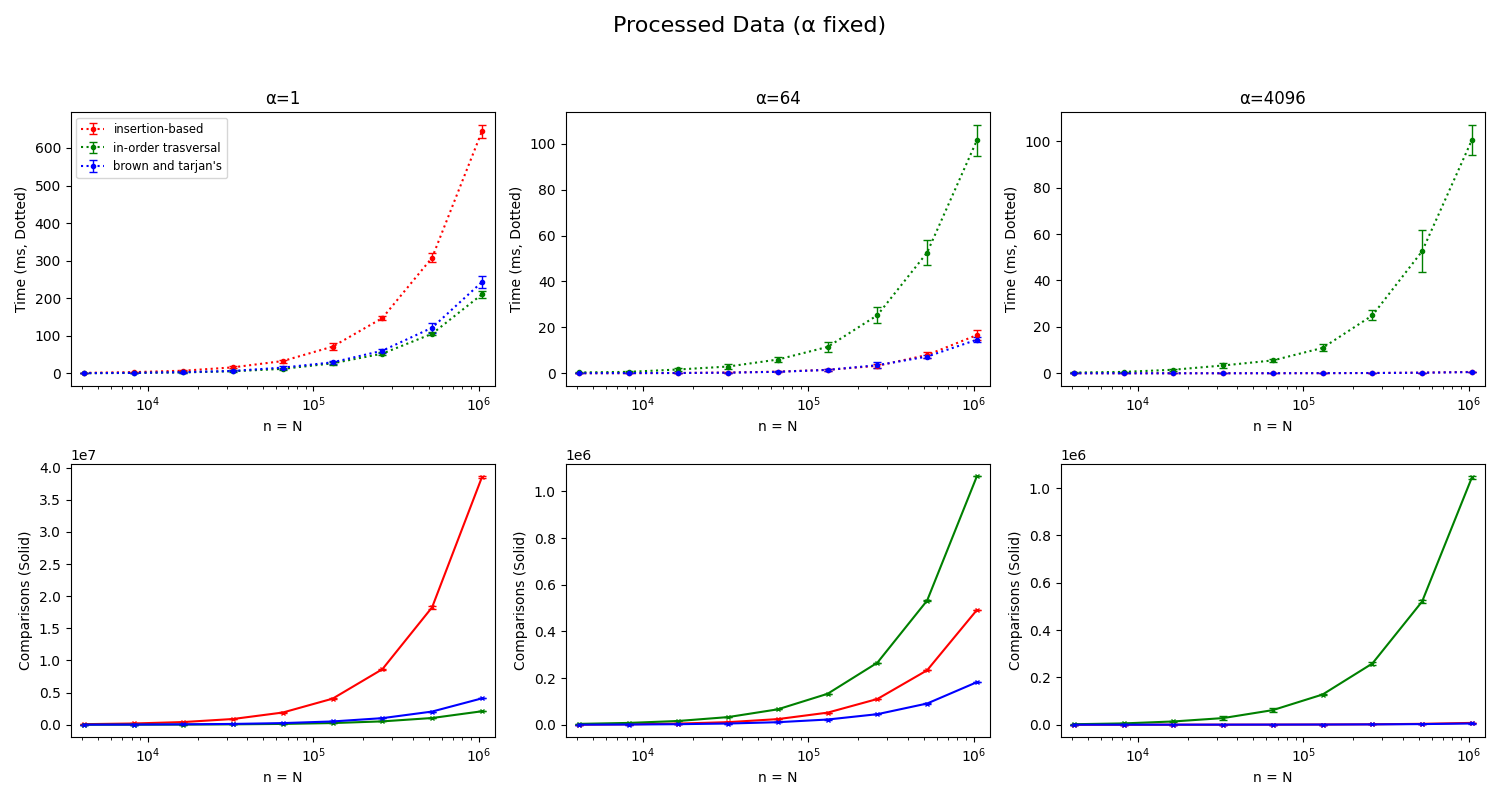
\includegraphics[width=\textwidth]{figure/Processed1.png}
    \caption{Processed data ($\alpha$ fixed)}
    \label{fig.proc1}
\end{figure}

\begin{figure}
    \centering
    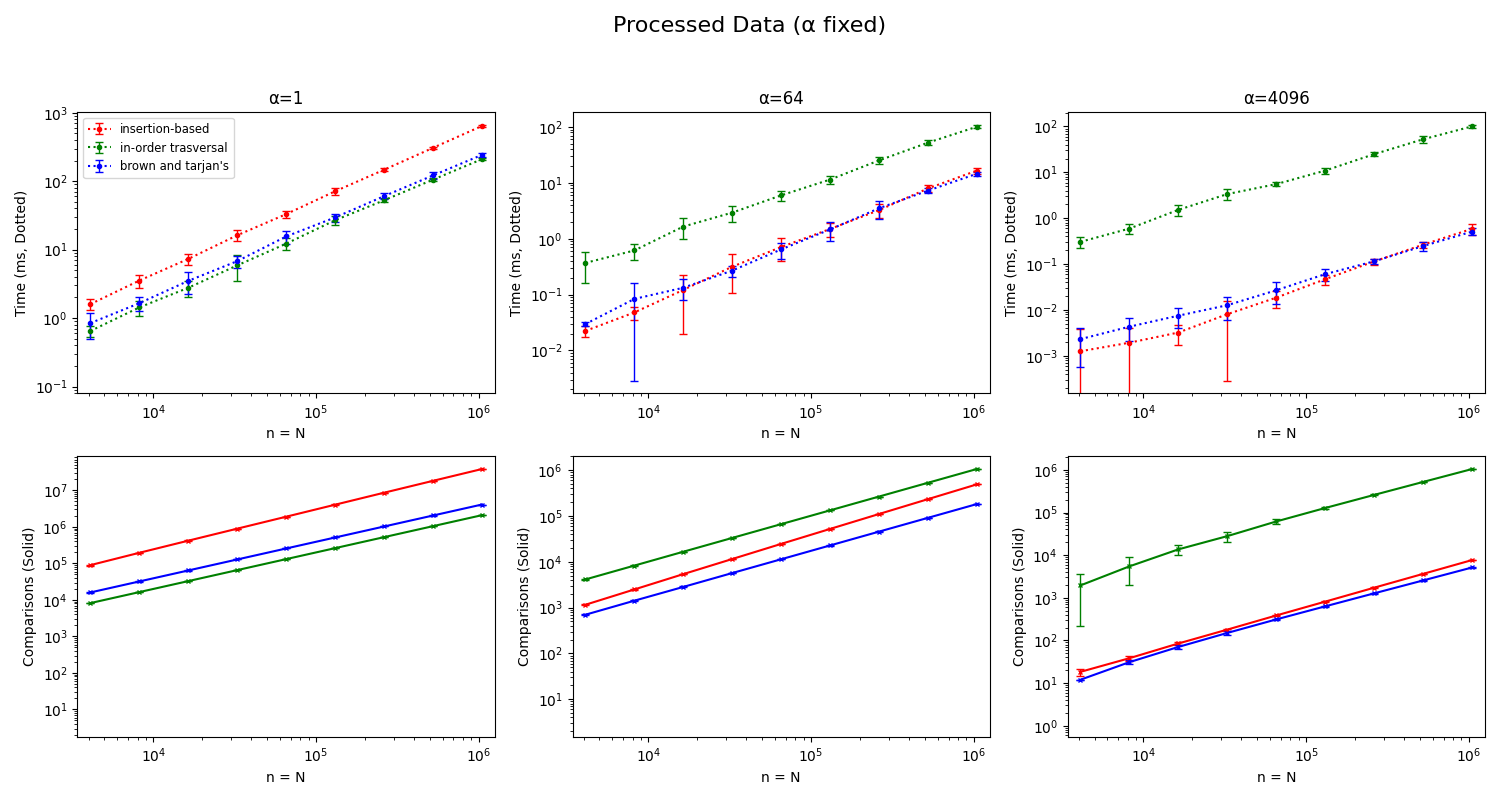
\includegraphics[width=\textwidth]{figure/Processed1(log).png}
    \caption{Processed data ($\alpha$ fixed) (both axis on log scale)}
    \label{fig.proc1log}
\end{figure}

\begin{figure}
    \centering
    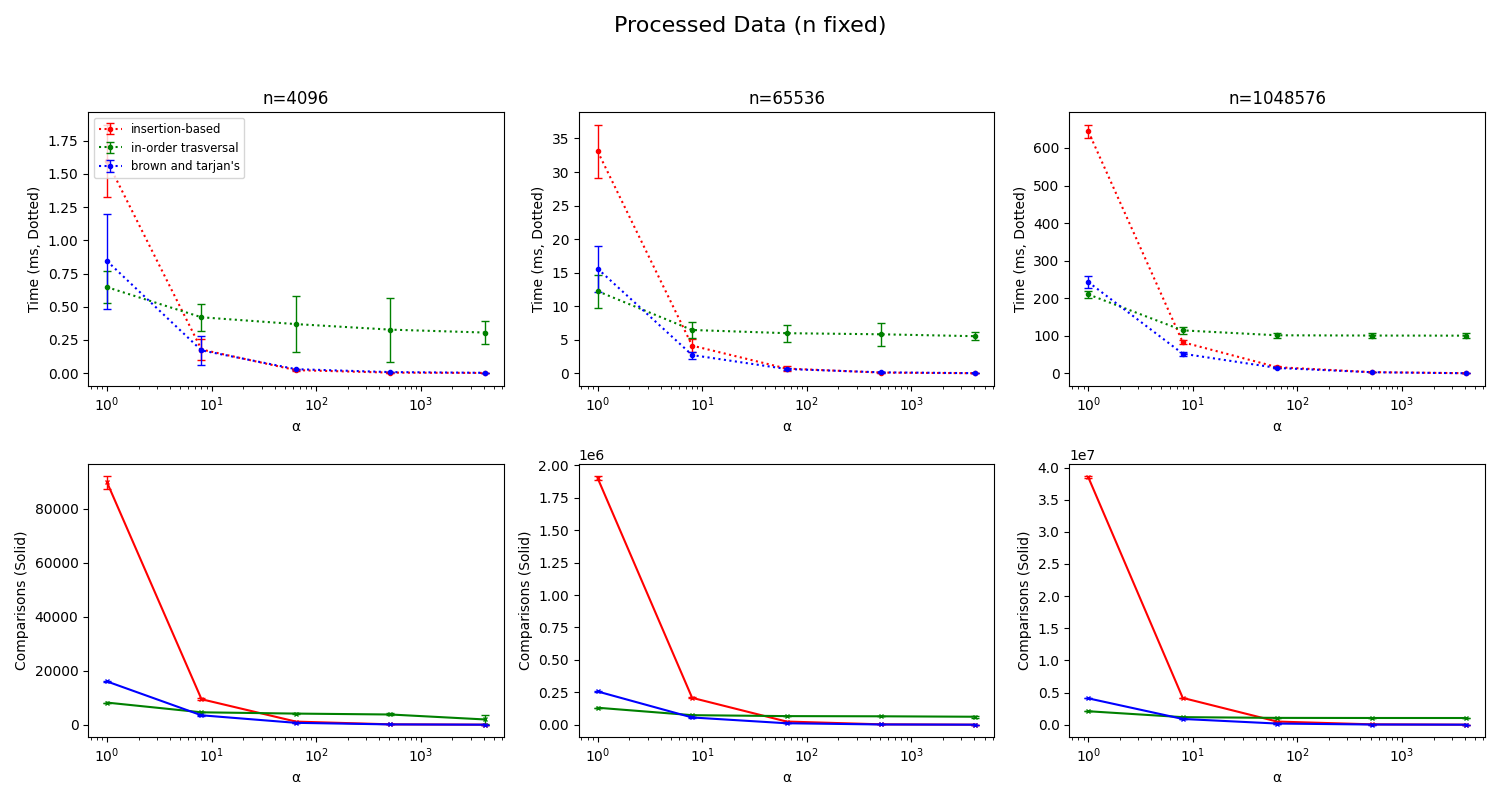
\includegraphics[width=\textwidth]{figure/Processed2.png}
    \caption{Processed data ($n$ fixed)}
    \label{fig.proc2}
\end{figure}

\section{Discussion and Conclusion}

\subsection{Correlation between $n$ and cost}

We can find clear trends from the graphs. In Figure \ref{fig.proc1}, we can see that the cost of the algorithm all increases as the total data size $n$ increases. It can be noticed that if we draw both axes in logarithmic scale, as is shown in Figure \ref{fig.proc1log}, the linear trend is more obvious. When $\alpha$ is fixed, the cost of three algorithms all increases linearly with the total data size $n$.

However, their rate of increase differs when $\alpha$ is different. For experiment where $\alpha = 1$, which means the sizes of both tree are the same, we can notice that both the time cost and the number of comparison of insertion-based algorithm is significantly higher than the other two algorithms, shown by a clear skyrockting trend in the graph. 

It can be also noticed that the despite having very significant disadvantage in number of comparison, the insertion based algorithm does not perform as bad as in the time. This might be because iteration through the smaller tree, which is obviously costly in this case as the tree takes up half the data, significantly costs time but not comparison.

On the contrary, for experiment where $\alpha = 64$, which means a small tree is being inserted to a significantly larger tree, the in-order trasversal algorithm become the most costly, with both the time cost and number of comparisons skyrockting. It can also be noticed that Brown and Tarjan's algorithm have smaller number of comparisons than the insertion-based algorithm, but similar cost in time. This might be because the cost of maintaining the path is quite significant. This implies if the cost of comparison is larger, like comparing the lexographical order of the strings, Brown and Tarjan's algorithm's advantage will be more obvious. These trends are even more significant when $\alpha = 4096$.

There is also abnormal large error bar when both axes are drawn in log scale, which results from the exageration of the error bar at small values, since $\log x$ is more steep than $x$ when $x$ is small.

\subsection{Correlation between $\alpha$ and cost}.

We can also find the advantage area of each algorithm in Figure \ref{fig.proc2}. As is shown in the graph, insertion-based algorithm shows the least consistent performance when $\alpha$ differs, with significant higher cost when $\alpha = 1$ and have lower cost when $\alpha$ is bigger. In-order transversal algorithm performs the best when $\alpha$ is small, but the cost reduces very slowly when $\alpha$ is bigger. This make it the algorithm with the most consistent performance. Brown and Tarjan's algorithm performs slightly inferior to in-order transversal algorithm when $\alpha$ is small, and performs almost as well as the insertion-based algorithm when $\alpha$ is large. This made it the best algorithm overall. It can be also noticed that three algorithms' performance is quite close when $\alpha \approx 8$.

The trend is almost the same throughout the graphs except for different scales, $\alpha$ is the only factor determining which algorithm is the optimal.

The error bars when $n$ is small are significantly larger. The apparent instability for small $n$ reflects the fact that the algorithm's asymptotic behavior is masked by constant factors and system-level effects.

\section{Evaluation}

% Perhaps add Pearson's r^2

The experiment is conducted successfully with sufficient data and supports our hypothesis. Test data incoporated a large number of trials and a wide range of independent variables, making the experiment more robust. The results are reproducible and consistent with the hypothesis. However, there is still room for improvement.

Limitations and improvements:

\begin{itemize}
    \item \textbf{Costly \texttt{new} and \texttt{delete} operations}: For the simplicity of implementation, \texttt{new} and \texttt{delete} oprations are used to create and free nodes in the tree. Repetitive \texttt{new} and \texttt{delete} operations are expensive, risky and inconsistent with modern C++ standard \cite{meyers-2014}. A better implementation can be modern pointers and/or memory pool to avoid extra time cost.
    \item \textbf{Cache warmup and memory fragmentation control}: First several trials may be slower due to lack of cache warmup, later trials may be slower due to memory fragmentation. A better implementation is to run serveral warmup trials and use memory pool to avoid memory fragmentation.
    \item \textbf{Regular independent variables}: To avoid floating point calculation when calculating data size, the powers of $2$ are used as the sizes of the sequence generated. However, this results in a complete binary tree after tree construction, which is not always the case in practice. A better implementation is to use more independent variables and generate them randomly.
    \item \textbf{O(1) comparison of \texttt{int}}: Only integer values whose comparision is $O(1)$ are put into the binary search trees. In many cases, the comparison can be more costly like in lexographical order, floating point number comparison, big numbers or their ratios, etc. In these cases, the cost of logic or memory operations can be more insignificant compared to the cost of comparison, which means reducing the number of comparison is of greater priority. This can result in significantly different performance under the same data scale, as is discussed before. It would be better if more data types other than integer are used.
    \item \textbf{Fully shuffled dataset}: Only cases where the data is fully shuffled are considered. In many cases, the data is not purely random. Some algorithm may run well for random data but not every trial, like treap without random priority. When merging two instances of ordered data structures, elements in one instance may be significantly smaller than the other, in which case the performance can be different. Cases like this should be investigated as well. 
    \item \textbf{Limited trials and independent variable range}: The experiment is conducted with a limited number of trials and a limited range of independent variables, due to the time limit and poor performance of the device. Some properties that can only be found with large $n$ or certain dataset may not be investigated. It would be better if more trials and larger independent variable ranges are used with a better device.
    \item \textbf{No multithreading considered}: This essay did not discuss possible multithreading improvement of the algorithms. % Because I'm not able to :-(
\end{itemize}

\bibliographystyle{apacite}
\bibliography{cit.bib}

\section*{Appendix A Test environment}

\begin{longtable}{@{}ll@{}}
\caption{Test environment} \label{tab.env} \\
\textbf{Device:} & Laptop \\
\textbf{CPU:} & Intel(R) Core(TM) Ultra 7 155H (1.40 GHz) \\
\textbf{Memory:} & 32GB \\
\textbf{OS:} & Windows 11 24H2 26100.6584 \\
\textbf{Compiler (C++):} & g++ 15.2.0 (algorithm implementation and timing) \\
\textbf{Compiling Command:} & \texttt{g++ test.cpp -o test -std=c++17 -O0 -Wall} \\
\textbf{Interpreter:} & Python 3.12.2 (graphing) \\
\end{longtable}

\section*{Appendix B Algorithm implementation}

%\lstinputlisting[
%    caption={VectorSet},
%    label=lst:vecsetheader
%]{code/vector_set.h}

\lstinputlisting[
    caption={avl\_set.h},
    label=lst.avlsetheader
]{code/avl_set.h}

\lstinputlisting[
    caption={test.cpp},
    label=lst.test
]{code/test.cpp}

% Working directory info:
%PS D:\code\ee> tree /f /a
%Folder PATH listing for volume Data
%Volume serial number is 5ADF-3FB3
%D:.
%|   cit.bib
%|   essay.bbl
%|   essay.dvi
%|   essay.pdf
%|   essay.synctex.gz
%|   essay.tex
%|
%\---code
%        avl_set.h
%        test.cpp
%        vector_set.h

\end{document}